% Gemini theme
% https://github.com/anishathalye/gemini

\documentclass[final]{beamer}

% ====================
% Packages
% ====================

\usepackage[T1]{fontenc}
\usepackage{lmodern}
\usepackage[size=custom,width=120,height=72,scale=1.0]{beamerposter}
\usetheme{gemini}
\usecolortheme{durham}
\usepackage{graphicx}
\usepackage{booktabs}
\usepackage{tikz}
\usepackage{pgfplots}
\pgfplotsset{compat=1.14}



\usepackage{subcaption}
\graphicspath{ {./Figures/} }
\newsavebox{\measurebox}
\usepackage{code}
\usepackage{wrapfig}
\newcommand{\proc}[1]{\textit{#1}}
% ====================
% Lengths
% ====================

% If you have N columns, choose \sepwidth and \colwidth such that
% (N+1)*\sepwidth + N*\colwidth = \paperwidth
\newlength{\sepwidth}
\newlength{\colwidth}
\setlength{\sepwidth}{0.025\paperwidth}
\setlength{\colwidth}{0.3\paperwidth}

\newcommand{\separatorcolumn}{\begin{column}{\sepwidth}\end{column}}

% ====================
% Title
% ====================

\title{Using a compiler based approach, FLAT, to accelerate Finite Volume kernels within ExaHyPE}

\author{Jack Slingsby}

%\institute[shortinst]{\inst{1} Some Institute \samelineand \inst{2} Another Institute}

% ====================
% Footer (optional)
% ====================

\footercontent{
  %\href{https://www.example.com}{https://www.example.com} \hfill
  %Middle Footer \hfill
  %End footer
  Durham University
  }
% (can be left out to remove footer)

% ====================
% Logo (optional)
% ====================

% use this to include logos on the left and/or right side of the header:
 \logoright{
\includegraphics[height=7cm]{Figures/DurhamUniversityLogo_WHITE.png}}
% \logoleft{\includegraphics[height=7cm]{logo2.pdf}}

% ====================
% Body
% ====================

%\begin{alertblock}{Hard Highlighed block}\end{alertblock}
%\begin{exampleblock}{Soft Highlighted Block} \end{exampleblock}

\begin{document}

\begin{frame}[t]
\begin{columns}[t]
\separatorcolumn

\begin{column}{\colwidth}

  \begin{block}{Background}

    % PDEs - what they are
Many physical phenomena can be described by partial differential equations (PDEs) including:  seismic wave propagation \cite{earthquakePDE}, fluid dynamics \cite{exahype}, and relativistic astrophysics \cite{relativisticPDE}.
As such, PDE solutions can have an important real world impact by, for example, improving tsunami modeling \cite{tsunamiPDE}.


Analytical PDE solutions are challenging to derive, and general solutions for any initial conditions or boundary conditions do not exist.
Instead, we rely on numerical methods to calculate approximate solutions.
However, numerical methods are computationally intensive; increasing the size of the problem, or the accuracy of the solution, increases the computational work required.
Many real world problems require billions of degrees of freedom to model.
The sheer scale of these computations requires the use of high performance computing (HPC), where algorithmic advances and supercomputers make these problems tractable.

In HPC, there are 2 ways to increase computational throughput, either by using more hardware, or by using available hardware more efficiently.
Supercomputing hardware is ever improving, and exa-scale systems are on the horizon.
However, relying on more hardware runs into cost and availability issues.
Therefore, optimising code to better use the hardware is often preferable.
In HPC code there are many levels at which optimisation can occur, one of the most fundamental being improving the throughput of a single core.
There are many example in literature of this having a significant effect on the performance of HPC code \cite{YATeTo,seisolPFLOP,codegen_dg_SIMD}, and this will be the area of optimisation we explore.     

% Exhaype - what it is
Our focus will be on the per core performance of Finite Volume (FV) kernels used to solve PDEs within ExaHyPE (an Exascale Hyperbolic PDE Engine) \cite{exahype}.
Implementing a HPC FV solver is a non-trivial task, and can take research teams months, or even years \cite{tensorChemistry}.
This is the problem that ExaHyPE solves by providing a generalised framework to create solvers for many different problems.
ExaHyPE's domain is linear and non-linear hyperbolic systems of PDEs written in first order form.

The Peano framework \cite{PeanoFramework} lies at the heart of ExaHyPE.
This is responsible for dividing the spacial domain into smaller patches and distributing these patches across computing resources.
Every patch is updated by a single core using the FV scheme.
It is this update process we will optimise.

To use ExaHyPE, a user begins by describing their problem to the ExaHyPE toolkit using a Python interface.
A user will specify information such as: how many unknowns and auxillary variables are used; whether their problem uses a non-conservative product (NCP); what numerical scheme they want to use; if they want to use fixed or adaptive time stepping; how frequently the solution should be plotted; and more.
This is used by the ExaHyPE toolkit to generate a project.
This project is primarily populated by glue code that invokes ExaHyPE, however there are a few placeholder functions that need to be filed in by the user.
These placeholder functions are used to describe the PDE, calculating: flux, eigenvalues, initial conditions, boundary conditions, and non-conservative products (if applicable).
Upon completing these placeholder functions, the project can be compiled and run on systems ranging from a laptop to a supercomputer.

% Exahype - benifits of exahype (fast flexible, friendly)
ExaHyPEs is designed to be fast, flexible and user-friendly; allowing users to create fast programs to solve a wide range of problems while requiring minimal effort from the user.
However, being flexible and user friendly often limits the opportunities for optimistations, especially at the boundary between user and engine code.
In this paper we set out to solve this problem using our compiler based approach \phlat, so called for the Flat Long and potentially Transformed code it produces.
\phlat aims to bridge the gap in ExaHyPE between being flexible and friendly, while producing fast C++.  

\phlat{}'s approach to optimisation is to generate C++ that \texttt{g++}, \texttt{clang++}, \texttt{ipcx}, e.t.c. are more capable of optimising.  
Namely, \phlat can be used to generate monolithic functions that are tens of thousands of lines long.
In this paper we investigate the performance of these kernels and thus how well they are optimised by compilers.

Relying on the compiler for optimisations is often taken for granted, simply appending an \texttt{-O3} flag to the compiler arguments can increase the performance of code by orders of magnitude.
And using vendor specific compiler, like Intel's \texttt{ipcx}, offers code hardware specific optimisation.
As such, relying primarily on compilers for optimisation is a promising direction for exploration.
Also looking to the future, we see that compilers are only getting more advanced.
Most recently the application of Machine Learning within compilers is being explored \cite{compiler-ml-opt,lots-of-compiler-options}, and development environments such as CompilerGym \cite{compiler-gym} suggest this area of research is set to expand.
Thus suggesting that relying on compilers also offers an aspect of longevity to optimisations as well.

% what is in each section
In the next section we go into depth about what problem \phlat solves within ExaHyPE, followed by discussing similar compiler based approaches.
In Section \ref{sec:methodology} we explain the architecture of \phlat and how it is used to generate compute kernels.
In Section \ref{sec:results} we will discuss the performance of kernels generated along with the practicalities of using \phlat. 

  \end{block}

  \begin{block}{Problem}

   Nam vulputate nunc felis, non condimentum lacus porta ultrices. Nullam sed
    sagittis metus. Etiam consectetur gravida urna quis suscipit.

    \begin{itemize}
      \item \textbf{Mauris tempor} risus nulla, sed ornare
      \item \textbf{Libero tincidunt} a duis congue vitae
      \item \textbf{Dui ac pretium} morbi justo neque, ullamcorper  
    \end{itemize}

    Eget augue porta, bibendum venenatis tortor. 

  \end{block}
  
  \begin{block}{Solution Approach}

   Our approach primarily relies on the optimising power of conventional compilers such as \textit{gcc}.
If we can \textbf{present the conventional compiler with code that it is better able to optimise}, then our compute kernels will receive a performance increase that is portable across many systems. 
To do this we created the FLAT compiler.
FLAT takes problems encoded an Directed Acyclic Graphs, and generates \textbf{Flat Long And potentially Transformed code}.
Users are able to implement additional code transforms if they desire, however it is not required.
The output of FLAT is then passed to a conventional compiler to be optimised.
 

  \end{block}

\end{column}

\separatorcolumn

\begin{column}{\colwidth}

  \begin{block}{Compiler Architecture}

    \textbf{DAG}: Our compiler, FLAT, takes a DAG (Directed Acyclic Graph) as an input.
Every node in the DAG has input and output ports.
Nodes are either a primative operation such add addition or subtraction.
Or nodes are DAGs, allowing a nested structure. 

\textbf{IR}: After applying DAG transforms, FLAT transforms the DAG into a code like Internal Representation (IR).
It is easier to generate code from this IR than directly from the DAG.
Our IR comes in 2 flavours, loose and tight.
The loose IR is much more relaxed, using simple function signatures and allowing special types of temporary variables.
The tight IR is much stricter and closer to output code and requires the use of features such as complex function signatures.

\newsavebox{\looseIRlisting}
\begin{lrbox}{\looseIRlisting}% Store first listing
\minipage{.68\textwidth}
\begin{lstlisting}
define VOID @kernel (%in0, %in1) (%out0, %out1):
	%tmp1 = %in0
	%tmp2 = %tmp1 * %tmp1 * %tmp1
	%tmp3 = %in1
	%tmp4 = %tmp2 + %tmp3
	%tmp5 = %tmp4
	%tmp6 = %tmp2 - %tmp3
	%tmp7 = %tmp6
	%out0 = %tmp5
	%out1 = %tmp7
\end{lstlisting}
\endminipage
\end{lrbox}



\newsavebox{\tightIRlisting}
\begin{lrbox}{\tightIRlisting}% Store first listing
\minipage{.68\textwidth}
\begin{lstlisting}
define VOID @kernel (new #list(in), new #list(out)):
	new #tmp2 = #in[0] * #in[0] * #in[0]
	#out[0] = #tmp2 + #in[1]
	#out[1] = #tmp2 - #in[1]
	<return nothing>
\end{lstlisting}
\endminipage
\end{lrbox}

\begin{figure}
\centering

\sbox{\measurebox}{%
  \begin{minipage}{.68\textwidth} \centering
        \subfloat[Loose IR]{\label{fig:figB}\usebox{\looseIRlisting}}
        \vspace{1em}
        \subfloat[Tight IR]{\label{fig:figC}\usebox{\tightIRlisting}}
  \end{minipage}
}

\usebox{\measurebox}\qquad
    \begin{minipage}[][\ht\measurebox][c]{.26\textwidth}
      \subfloat[Input DAG]{\label{fig:loose_tight_dag}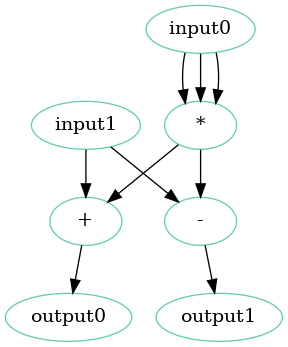
\includegraphics[width=\textwidth]{tight_vs_loose.png}}
       
    \end{minipage}
\caption{Example of the difference between a loose IR and tight IR. Figure \ref{fig:loose_tight_dag} shows the corresponding input DAG.} 
\label{fig:tight_loose}
\end{figure}

    \begin{figure}[h!]
    \begin{center}
        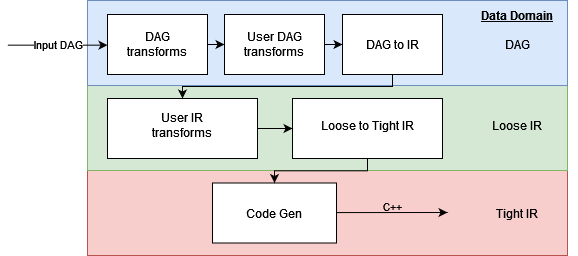
\includegraphics[width=.7
        \textwidth]{comp-arch.png}
        \caption{Overview of FLAT's architecture.}
        \label{fig:arch}
    \end{center}
\end{figure}

  \end{block}
  \begin{block}{Compiling FV Kernels}

   A user begins by creating DAGs for the Problem Definition (i.e. flux, ncp, source terms, max eigenvalue functions).
A user then wraps these DAGs in builder functions (A function that when called returns a new version of their DAG).
These builder functions are then passed to a \proc{Patch Update} builder function, which is provided by the engine.
\proc{Patch Update} uses the user's DAGs numerous times, and creates a new user DAG for every single use.

The final \proc{Patch Update} DAG is passed to the FLAT compiler.
Here compiler transforms are preformed, and optional user transforms are preformed.
The final C++ output is typically 1000s to \textbf{10,000s of lines long}, and can be used as a direct replacement in an ExaHyPE project.



  \end{block}

\end{column}

\separatorcolumn

\begin{column}{\colwidth}

  \begin{block}{Results}

   We used 3 test problems: Euler Equations in 2D and 3D (Euler 2D, Euler 3D), and the shallow water equations (SWE).
These 3 problems are provided as examples within the ExaHyPE repository, and those kernels were used as control kernels which we refer to as \textit{default}.
We then recreated these kernels as DAGs and used FLAT to compile them into C++.
Our first method for comparison is a simple synthetic benchmark that measured how many iterations per second a kernel could preform on a fixed input.  

\begin{table}
    \centering
    \begin{tabular}{lllrr}
\toprule
Problem & Kernel & System & Iterations per ms & Speedup \\
\midrule
Euler 2D & default & Intel & 152.90 & - \\
Euler 2D & compiled & Intel & 2486.15 & 16.26 \\
Euler 3D & default & Intel & 50.20 & - \\
Euler 3D & compiled & Intel & 603.29 & 12.02 \\
SWE & default & Intel & 150.98 & - \\
SWE & compiled & Intel & 2313.76 & 15.32 \\
Euler 2D & compiled & AMD & 3150.51 & 8.66 \\
Euler 3D & compiled & AMD & 663.42 & 8.62 \\
SWE & compiled & AMD & 2874.82 & 11.38 \\
\bottomrule
\end{tabular}
 
    \caption{Performance of compiled kernels against default kernel in a synthetic benchmark.} 
\end{table}

Our compiled kernels preformed well, achieving approximately an order of magnitude speedup over the \textit{default} kernels.
This translated to a \textbf{speedup of 5\% - 15\% in ExaHyPE}, which was to be expected for our memory bound test problems.

We also compared a hand optimised kernel against a compiled kernel. 
\begin{table}
    \centering
    \begin{tabular}{lrrr}
\toprule
Kernel & Iterations per ms & Speedup vs Default & Speedup vs Handmade \\
\midrule
default & 363.67 & 1.00 & 0.27 \\
handmade & 1364.63 & 3.75 & 1.00 \\
compiled & 3150.51 & 8.66 & 2.31 \\
\bottomrule
\end{tabular}
 
    \caption{Performance of kernel optimised by hand against compiled kernel.}
\end{table}

We found a \textbf{$2.3\times$ speedup of compiled kernels over manual optimisation}.
This was due to \textbf{increased automatic SIMD vectorization} by the \textit{aocc} and \textit{ipcx} compilers.
Using the MAQAO static analysis tool \cite{MAQAO}, we observed a 60\% floating point vectorization ratio which was almost double that of the hand optimised kernels.

  \end{block}

  \begin{block}{Conclusion}

    This paper presents \phlat as a method for bridging the gap in ExaHyPE, between being flexible and user-friendly, while producing fast C++.
\phlat delivers on producing fast C++, producing kernels that were up to $16\times$ faster than kernels currently used in ExaHyPE.
This speedup was enabled by \phlat{}'s dynamic code generation approach, that produced monolithic compute kernels, thousands of lines long.
Compiled kernels even out preformed a hand optimised kernel, owing to better automatic vectorisation of the compiled kernels while using the \texttt{-ffast-math} flag.

As would be expected, this speed up didn't directly carry over to the performance of our memory bound test problems in ExaHyPE.
Here, we saw speedups of $5\% - 15\%$, the best being in the Euler 3D test problem which is the most computationally intense of the 3 test problems.

This leads on to \phlat{}'s shortcomings.
The nested structure of DAGs in \phlat mirrors the modularity that users of ExaHyPE currently experience.
However, the cumbersome process of creating a DAG edge by edge is not user friendly, and limits the size of DAGs that can be reasonably created.
The development of front end to \phlat such as via a DSL or SymPy interface, would help mitigate these issues and allow \phlat to tackle larger problems.

The behaviour of \phlat on large problems is unknown, and it may be the case that \phlat, in its current state, is unsuitable for large problems.
However, the improvements witnessed on small test problems does warrant the development of a front end, so \phlat{}'s performance on larger problems can be explored.

Furthermore, the switch from static to dynamic code generation in ExaHyPE opens up many more avenues for exploration.
In \phlat users can define their own domain specific transforms, which may prove a useful feature.
And further afield, dynamic code generation may allow for CPU/GPU agnostic code, which is an interesting direction for further exploration.



  \end{block}

  \begin{block}{References}

    \nocite{*}
    \footnotesize{\bibliographystyle{plain}\bibliography{poster}}

  \end{block}

\end{column}

\separatorcolumn
\end{columns}
\end{frame}

\end{document}
